\documentclass[12pt, a4paper]{article}

%Paketler ve kullaımları
\usepackage[ddmmyyyy]{datetime}
\usepackage{graphicx}
\usepackage{ragged2e}
\usepackage{float}
%overrides
\renewcommand{\dateseparator}{.}
\renewcommand{\figurename}{Şekil}
\renewcommand{\refname}{Kaynaça}
\restylefloat{figure}

%ayarlamalar
\title{Metinden görsel oluşturma projesi}
\author{Mustafa Erdogdu}
\date{10.06.2024}
\graphicspath{ {./images}}
\floatstyle{boxed} 


\begin{document}
	
	\begin{figure}
		\centering
		
\includegraphics{ksbu.png}
	\end{figure}
	
	\maketitle
	
	\noindent
	\begin{center}
		\textbf{Abstract}
	\end{center}
 	Bu pojeyi oluşturmada temel amaç insanların hayal ettiği şeyleri muazzam uğraşlar vermeden görsel karşılıklarını alabilmelerini sağlamak. Bu hayal edilen şey belki bir rüya, belki bir senaryo veya geçmişte yaşadığı bir anı olabilir. Tabiki projenin ilk kısmı bu kadar detaylı görseller üretme konusunda yetersiz olsa da bu projenin belki de yapıtaşı olan “hayal etmek” kelimesi ilerleyen çalışmalarda böyle kompakt bir çalışma yapmak için fırsat tanıyor.   
 	Bu çalışmada yapılanları adım adım açıklayacak olursak başlangıç olarak görsel ayrıştırma modeli oluşturuldu daha sonra metin analiz modeli oluşturuldu. Bu iki model henüz birleştirilemedi ama metinden görsel oluşturma işlemi hazır görsel apileri kullanılarak sağlandı. Tasarlanan proje stable diffision modeline benzer şekilde üretilecekti ama projede ilerledikçe bu çizgiden biraz dışarı çıkıldı. stabble diffisionda metinden görsel üretme işlemi gürültüden adım adım görüntü oluşturmak ile mümkün ama bu projede görsel oluşturmak için doğrudan metin vektörü kullanılması amaçlanıyor.
 	Sonuçlar gösterdi ki metinden görsel oluşturma projesi beklenilenden çok daha kompleks bir projeymiş. Kullanılan mimariler ve algoritmaları ortak bir projede birleştirmek için 10 haftalık proje süresi yeterli gelmedi. İlerleyen süreçte bu projeyi bitirmek için gerekli çalımlara devam edilecektir.
	
	\section{Giriş}
		Bu projede, hazır kodlanmış Vgg16 modeli kullanılarak başka verilerile ile bir model eğitimi gerçekleştirildi ve modele çıkarım katmanları eklenerek görsel ayrıştırma modeli oluşturuldu. GoogleNews-vectors-negative300.bin veri kümesi kullanılarak kelime benzerliği bulma yöntemiyle manzara kelimeleri keşfedildi ve Word2Vec(W2W) modeliyle benzerlikler analiz edildi.Bu proje için oluşturulan metin veritabanındaki promtlar kullanılarak bir W2V gömme modeli oluşturuldu. Ayrıca, webden metin kazıyarak kelime bulutları oluşturuldu ve kullanıcı tarafından girilen kelimeye benzer kelimelerin grafiği çıkarıldı. Bu kelime vektörleri görsel modellerle eşleştirilip metinden görsel oluşturma projesinde kullanılmak üzere kaydedildi. Kullanıcının girdiği promt metin ön işleme adımlarıyla tek bir kelime vektörü haline getirildi ve Unsplash API'si kullanılarak bu promta göre görseller üretildi. Çalışmanın sonraki adımında Unsplash API yerine model.keras dosyası kullanılarak görseller üretilmesi hedefleniyor.
	
	\section{VERİ VE LİTERATÜR ARAŞTIRMASI}
	
	\subsection{Nlp(doğal dil işleme)}		
	Doğal dil işleme (NLP), bilgisayarlara insan dilini yorumlama, işleme ve anlama yeteneği veren bir makine öğrenimi teknolojisidir. insan dilini işlemek için hesaplamalı dil bilim, makine öğrenimi ve derin öğrenme modellerini birleştirir. NLP yazılımları, çeşitli uygulamalar için verileri hazırlamak adına belirteçlere ayırma, kök ayırma, kök çözümleme ve etkisiz kelimelerin kaldırılması gibi ön işleme tekniklerini kullanır.	 
	
	\subsection{Dikkate dayalı modelleme}	
	Dikkatte dayalı modeller , bir girdinin en önemli parçalarına odaklanmak ve bunları işlemek için kullanılan bir dizi model türüdür. Bu modeller, girdinin tümünü işlemek yerine, hangi parçaların en alakalı ve bilgilendirici olduğunu belirlemek için bir dikkat mekanizması kullanır.\cite{Dikkate-dayalı-modelleme}
	
	\subsubsection{Transfomatörler  nedir}	
	'Attention Is All You Need ' başlıklı makale transformatörleri tanıtıyor. Başlığın da belirttiği gibi, daha önce gördüğümüz dikkat mekanizmasını kullanıyor.\cite{transformator2} kelimeler arasındaki uzun mesafeli bağımlılıkları modellemek için kullanılan bir tür dikkat mekanizmasıdır. Transformatörler, bu mekanizmayı, bir metnin veya kodun farklı parçaları arasındaki ilişkileri öğrenmek için kullanır. Transformer  iki parça (Encoder ve Decoder) yardımıyla bir diziyi diğerine dönüştürmeye yarayan bir mimaridir\cite{transformator1}\\
	
	\subsubsection{Gan}		
	GAN, derin öğrenme alanında kullanılan bir yapay zeka (AI) modelidir. GAN, iki ayrı yapay sinir ağından oluşur \\
	•	Üretici (Generator): Bu ağ, girdi olarak rastgele gürültü alır ve gerçek verilere benzeyen yeni veriler (resimler, sesler, metinler vb.) üretmeye çalışır.\\
	•	Ayırt Edici (Discriminator): Bu ağ, gerçek verileri üretici tarafından oluşturulan verilerden ayırt etmeye çalışır.\\
	GAN'lar, birbirleriyle "çekişerek" öğrenirler. Üretici, ayırt ediciyi aldatmaya çalışarak daha gerçekçi veriler üretmeye çalışır. Ayırt edici ise, verilerin gerçek olup olmadığını daha iyi ayırt etmeye çalışır. Bu rekabet sayesinde, her iki ağ da zamanla gelişir ve daha iyi performans gösterir.\cite{Gan-nedir}\\
	
	\subsection{Stable Video Diffuzyon ve Gan farklılıkları}
	•Stable Video Diffusion, gürültü difüzyon ve ters difüzyon modelleriyle çalışır.\\
	•GAN, birbirleriyle rekabet eden üretici ve ayırt edici ağlardan oluşur.\\
	•Stable Video Diffusion , GAN'lara kıyasla daha az hesaplama gücü gerektirir ve bu nedenle daha hızlı çalışır.
	•Her iki model de yapay zeka görüntü işlemede kullanılsa da, farklı çalışma prensiplerine sahiptir.\\
	•Stable Diffusion: Portre resimleri oluşturma, arka planları değiştirme, nesne ekleme veya kaldırma gibi görüntü düzenleme uygulamalarında kullanılır.
	•GANs: Daha çok yaratıcı görüntü oluşturma, nesnelerin 3 boyutlu modellerinin oluşturulması gibi alanlarda tercih edilir. \cite{svd}
	
	\subsection{Gail}
	GAIL,  yapay zeka alanında kullanılan bir derin öğrenme tekniğidir. Bu teknik, diğerlerinden biraz farklı bir şekilde çalışan bir tür GAN olarak düşünülebilir. Gail spesifik konularda görsel oluşturma imkanı tanır .GAIL, belli bir tarzda veya stildeki verileri üretmekte daha başarılı olabilir.Dezavantajı ise metinden görüntü oluşturamaması.\\
	
	\subsection{Gürültüden görüntü oluşumu}	
	
	Metinden ses oluştumak için kullanıcının verdigi komutlar önce şekil \ref{Gurultu1} deki gibi gürültü olarak oluşur. Sonrasında komutlar doğrultusunda veri tabanındaki görsellerle kıyas yaparak adım adım şekil \ref{Gurultu2} ,şekil \ref{Gurultu3} ve şekil \ref{temiz}'e doğru ilerleyerek görsel oluşumu sağlanır.				
	
	\subsection{doğal dil işleme(Nlp)}		
	Nlp, bilgisayarlara insan dilini yorumlama, işleme ve anlama yeteneği veren bir makine öğrenimi teknolojisidir. insan dilini işlemek için hesaplamalı dil bilim, makine öğrenimi ve derin öğrenme modellerini birleştirir. NLP yazılımları, çeşitli uygulamalar için verileri hazırlamak adına belirteçlere ayırma, kök ayırma, kök çözümleme ve etkisiz kelimelerin kaldırılması gibi ön işleme tekniklerini kullanır. 
	%\subsubsection{Kullanılan kütüphaneler ve işlevleri:}
	
	\subsection{Torch}
	Torch, bilimsel hesaplamalar yapmak için birçok araç sağlar. Özellikle tensörler üzerinde işlemler gerçekleştirmek için kullanılır. Tensörler, çok boyutlu diziler olarak düşünülebilir ve matrislere benzerler, ancak daha yüksek boyutlara sahip olabilirler.
	
	\subsection{TorchVision}
	Torchvision, PyTorch kütüphanesi için geliştirilmiş bir kütüphanedir. Görüntü işleme ve bilgisayarlı görü uygulamaları için önceden eğitilmiş modeller, veri kümeleri ve yaygın dönüşümler sunar. Bu da, bu tür uygulamaları geliştirmeyi ve prototiplemeyi büyük ölçüde kolaylaştırır.\\
	\textbf{Torchvision'un sunduğu bazı temel özellikler şunlardır:}\\
	Popüler Görüntü İşleme Modelleri: AlexNet, ResNet, VGGNet gibi önceden eğitilmiş ve kullanıma hazır görüntü işleme modelleri içerir.\\
	Geniş Veri Kümesi Seçeneği: ImageNet, CIFAR-10, MNIST gibi yaygın görüntü veri kümelerine erişim sağlar.\\
	Görüntü Dönüşümleri: Resim boyutlandırma, kırpma, döndürme, renk uzay dönüştürme gibi yaygın görüntü dönüşümlerini kolayca uygulamanızı sağlar.\\
	Ek Yardımcı Araçlar: Görselleştirme araçları, model optimizasyon araçları ve hata ayıklama araçları gibi ek yardımcı araçlar da sunar.
	\subsection{Gensim Kütüphanesi Ne İşe Yarar?}
	Gensim, doğal dil işleme (NLP) alanında kullanılan ücretsiz ve açık kaynaklı bir Python kütüphanesidir. Metin verisini analiz etmek ve işlemek için çeşitli araçlar ve algoritmalar sunar. Gensim'in temel işlevleri şunlardır:\\
	\textbf{Konu Modelleme:}\\
	Büyük metin kümelerini analiz ederek gizli temaları ve konuları otomatik olarak belirler.
	Farklı metin türleri için uygun konu modelleme algoritmaları sunar.\\
	\textbf{Kelime Vektörleme:}\\
	Kelimeleri anlamsal ilişkilerine göre sayısal vektörlere dönüştürür.
	Bu vektörler, kelimelerin anlamlarını ve ilişkilerini temsil etmek için kullanılabilir.\\
	\textbf{Benzerlik Bulma:}\\
	Metinler, kelimeler ve cümleler arasındaki benzerliği hesaplar.
	Bu bilgiler, metin sınıflandırma, özetleme ve öneriler gibi görevlerde kullanılabilir.\\
	\textbf{Sözlük İşleme:}\\
	Metinlerden kelime ve kelime öbeklerini otomatik olarak çıkarır ve bunları işler.
	Bu bilgiler, duygu analizi, anahtar kelime çıkarma ve metin özetleme gibi görevlerde kullanılabilir.\\
	\textbf{Anlamsal Analiz:}\\
	Metinlerin anlamlarını ve ilişkilerini analiz etmek için çeşitli araçlar ve algoritmalar sunar.
	Bu bilgiler, metin sınıflandırma, duygu analizi ve metin özetleme gibi görevlerde kullanılabilir.\\
	\textbf{Gensim'in Kullanım Alanları:}
	Haber ve blog yazılarını analiz etme
	Sosyal medya verilerini işleme
	Müşteri yorumlarını analiz etme
	Bilimsel makaleleri ve raporları analiz etme
	Otomatik metin özetleme ve çeviri
	Sohbet robotları ve sanal asistanlar geliştirme
	Bilgi arama ve öneri sistemleri oluşturma\\
	\textbf{Gensim'in Avantajları:}\\
	Kullanımı kolay ve öğrenmesi hızlıdır.
	Çok çeşitli NLP görevlerini destekler.
	Etkili ve ölçeklenebilir algoritmalar sunar.
	Geniş bir topluluk tarafından desteklenir.\\
	\textbf{Gensim'in Dezavantajları:}\\
	Bazı gelişmiş NLP görevleri için daha özel kütüphanelere ihtiyaç duyulabilir.
	Büyük metin kümelerini işlemek için zaman ve kaynak gerektirebilir.
	\textbf{Gensim'i Kullanmaya Başlamak:}
	Gensim'i kullanmak için Python'u ve NumPy gibi bazı temel kütüphaneleri yüklemeniz gerekir. Gensim'i pip kullanarak kurabilirsiniz:
	"pip install gensim"
	Daha fazla bilgi için Gensim'in resmi belgelerine bakabilirsiniz\cite{gensim}.
	Özetle, Gensim, metin verisini analiz etmek ve işlemek için güçlü ve çok yönlü bir araçtır. NLP alanında çalışanlar veya metin verisinden bilgi çıkarmak isteyenler için idealdir.
	\subsection{Gensim'de Kelime Vektörleme Nasıl Yapılır?}
	Gensim kütüphanesi, kelimeleri anlamsal ilişkilerine göre sayısal vektörlere dönüştürmek için çeşitli kelime vektörleme algoritmaları sunar. 
	
	
	
	\section{YÖNTEM}
	\textbf{Çalışmada kullanılan yöntem ve modeller}
	\subsection{Stable Video Diffusion nedir(SVD)?}	
	SVD, yapay zeka (AI) alanında bulunan ve metinsel açıklamalara dayanarak video oluşturmak için kullanılan bir modeldir. 2022 yılında piyasaya sürülen bu model, kısa sürede ilgi çekmiş ve video oluşturma alanında yeni ufuklar açmıştır.\cite{yakar2020yapay}\\			
	
	\subsubsection{Stable Video Diffuzyon ile Metinden Görsel Oluşturma Adımları}
	•	Oluşturmak istediğiniz görseli detaylı ve net bir şekilde anlatan bir metinsel açıklama hazırlayın.\\
	•	Açıklamada renkler, nesneler, arka plan, kompozisyon ve görsel stil gibi unsurları detaylandırmaya çalışın.\\
	•	Örneğin, "Bir deniz kenarında, gün batımında, palmiye ağaçlarının altında duran bir çift sallanan sandalye" gibi bir açıklama hazırlayabilirsiniz.\\
	•	Metinsel açıklamayı Stable Video Diffusion modelinin kabul ettiği bir formata dönüştürmek için bir metinden vektöre (text-to-vector) modeli kullanılır.CLIP veya VQ-VAE gibi metinden vektöre modeller, metinsel açıklamayı sayısal bir vektöre dönüştürerek modelin anlayabileceği bir formata dönüştürür.\\
	•	Model, metinsel vektörü kullanarak rastgele gürültüden başlayarak gerçekçi bir görüntü oluşturmaya başlayacaktır.\cite{yakar2020yapay}

	\subsection{Automatic1111 nedir}
	Automatic1111, Stable Diffusion isimli metinden görsele dönüştüren güçlü bir yapay zeka modelini kullanmak için kullanılan popüler bir grafik arayüzüdür (GUI). Stable Diffusion ile etkileşim kurmanızı kolaylaştırarak, metin açıklamalarına veya prompt olarak bilinenlere dayalı olarak kolayca görüntü oluşturmanıza olanak tanır.\cite{Automatic1111}
	
	\subsection{Civit ai nedir}
	Civit ai hazır eğitilmiş modellerri kulllanmamıza olnak sağlayan sitede.
	\cite{civitai}\cite{github1111}
	\subsection{kullanılan kodlar}
	\cite{mimari} numaralı kagle çalışmasından faydalanıldı
	
	\subsection{Transformer Mimari}
	\subsubsection{Transformer Mimari nedir}
	Transformer, Google AI tarafından 2017 yılında geliştirilmiş ve "Attention Is All You Need" isimli makalede sunulmuş bir derin öğrenme modelidir. Dikkat mekanizması ve kodlayıcı-çözücü mimarisi gibi özelliklerinden dolayı doğal dil işleme ve makine çevirisi gibi görevlerde oldukça başarılıdır. Transformer modeli,metinden görüntü oluşturmak, metinleri bir dilden diğerine çevirmek (Google Translate), metin üretmek (GPT-3), metin anlayışı (BERT) gibi birçok farklı görevde kullanılmaktadır. Dikkat mekanizması sayesinde uzun vadeli bağımlılıkları modelleyebilme, paralel işleme için uygun bir mimariye sahip olma ve farklı görevler için uyarlanabilme gibi avantajları vardır. Fakat RNN'lere kıyasla daha karmaşık bir mimariye sahip olması ve eğitimi için büyük veri kümeleri ve güçlü işlem gücü gerekli olması gibi dezavantajları da mevcuttur.\cite{transformator2}
	\subsubsection{Transformer Mimari katmanları}
	Şekil \ref{trasnformer}'de transformer mimari katmanları görülmektedir\\
	\begin{figure}
		\centering
		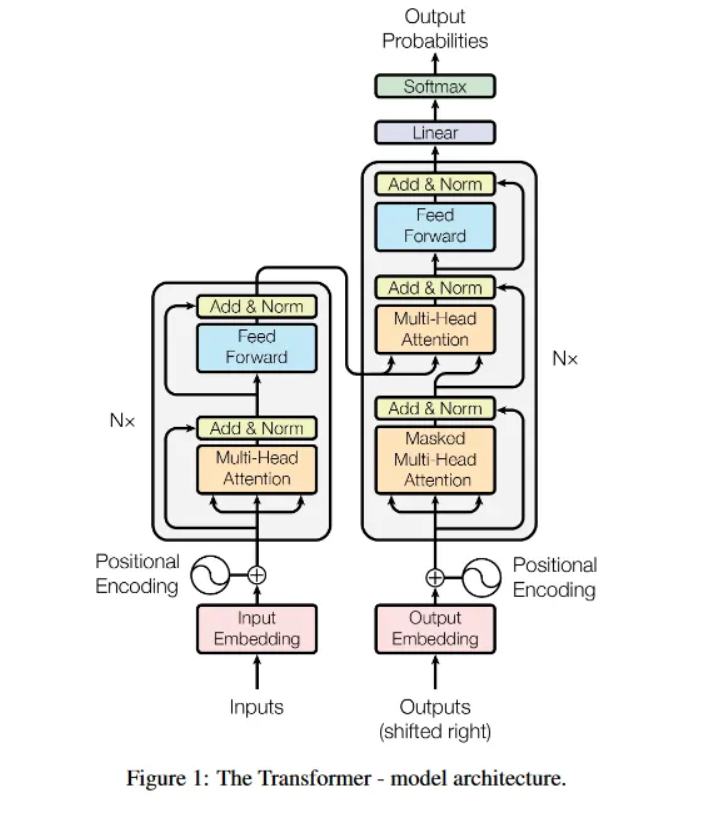
\includegraphics[width=12cm,height=8cm]{aaa.png}
		\caption{trasnformer Mimari}
		\label{trasnformer}
	\end{figure}	
	\textbf{Embedding Layer:} Bu katman kelimeleri veya diğer girdi simgelerini gerçek sayı vektörlerine dönüştürür.\\
	\textbf{Positional Encoding:} Transformatör mimarisi sıralı verileri işlemek için konumsal kodlama kullanır. Konumsal kodlama, dizideki her bir belirtecin konumunu belirten ek bilgidir.\\
	\textbf{Attention Layer:} Dikkat katmanı, girdi dizisinin hangi bölümlerinin çıktıyı oluşturmak için en önemli olduğunu belirler.\\
	\textbf{Feed-Forward Network (FFN):}  FFN, dikkat katmanından gelen bilgileri işler ve çıktı için bir tahmin üretir.\\
	\textbf{ Encoder and Decoder:} Transformatör mimarisi çoklu kodlayıcı ve kod çözücü katmanlarından oluşur. Her katman, giriş dizisini daha iyi işlemek ve daha doğru bir çıktı üretmek için bir önceki katmanın çıktısını kullanır.\cite{mimari}
	
	
	\subsection{Transformer Mimari nasıl çalışır}
	“İnput embedding” ile her satırı bir kelimeye karşılık gelen bir matrise çevirilecek . Sonra bu matris “encoder ” bloğuna girecek ve “multihead attention”, biriminden  geçerek ve yeni bir matris elde edilecek.
	Bu sırada “decoder(çözücü)” bloğuna bir adım önce yaptığımız görseller gelecek. Bu görseller yine matrise çevirilecek ve benzer işlemlere tabi tutulacak. Ancak bu sefer ikinci “multihead attention” biriminde girdi olarak “encoder” bloğunun çıktısı alınacak. “Decoder” bloğunun çıktısı son bir lineer fonksiyondan geçecek ve buradan alınan çıktılar softmax fonksiyonundan geçerek sonraki görünrtü için bize tahmin verecek.
	Transformerler bu işlemlerde dikkat mekanizmasını kullanıyor.Dikkat mekanızmasını basitçe anlatmak gerekirse,bir girdi dizisinin hangi bölümlerinin bir görev için en önemli olduğunu belirlemek için kullanılan bir tekniktir. Bu mekanizma, bir modelin girdi dizisinin tüm bölümlerine eşit dikkat etmesi yerine, belirli bölümlere odaklanmasını sağlar.
	\subsection{Transformer Mimari avantajları ve dezavantajları}
	\textbf{Transformer Mimarisi Avantajları:}\\
	•	RNN'lere kıyasla daha uzun metin dizilerini daha iyi işleyebilir.\\
	•	Kelimeler arasındaki uzun mesafeli bağımlılıkları öğrenebilir.\\
	•	Daha hızlı ve daha verimlidir.\\
	•	Farklı NLP görevlerine uyarlanabilir.\\
	\textbf{Transformer Mimarisi Dezavantajları:}\\
	•	RNN'lere kıyasla daha fazla veri ve işlem gücü gerektirir.\\
	•	Karmaşık bir mimaridir ve anlaması zor olabilir.\\
	
	\subsection{VGG16 Modeli Nedir?}
	VGG16, 2014 yılında Visual Geometry Group (VGG) tarafından geliştirilmiş bir konvolüsyonel sinir ağı (CNN) modelidir.
	
	\textbf{Özellikleri:} 				
	Görüntü sınıflandırma, nesne algılama ve bölgeleme gibi birçok görevde oldukça başarılıdır.\\
	16 katmandan oluşur ve bu katmanların 13'ü konvolüsyonel katmandır.\\
	Her konvolüsyonel katmandan sonra bir max pooling katmanı bulunur.\\
	Son katmanlarda ise tam bağlantılı katmanlar kullanılır.
	ImageNet veri kümesi üzerinde eğitilmiştir.\\
	1000 farklı nesne kategorisini sınıflandırabilir.\\
	
	\subsection{Çalışmada geliştirilen modeller}
	\subsection{Görüntü ayrıştırma modeli}
	Bu model veri setine ait  manzara görsellerini ayrıştırma için kullanılmak üzere geliştirild.
	
	\subsection{Word2Vec modeli}
		Metin analizi için geliştirilen Word2Vec, kelimeleri gerçek sayılardan oluşan vektörlere dönüştüren bir sinir ağları modelidir. Bu vektörler, kelimelerin anlamsal ilişkilerini ve benzerliklerini yakalamada oldukça etkilidir.	
	
	\subsection{metin modeli oluşturma adımları}
	\subsection{Metin kazıma(web scraping)nedir?}
	Metin kazıma , web sitelerinden veri toplama işlemidir. Bu, bir web sayfasının HTML yapısını analiz ederek belirli verileri çıkarmayı içerir. Python'da metin kazıma için en popüler kütüphanelerden bazıları BeautifulSoup, requests ve Selenium'dur. Aşağıda, BeautifulSoup ve requests kullanarak basit bir metin kazıma örneği verilmiştir.Bu çalışmada BeautifulSoup kullanıldı.Bunun sebebi BeautifulSoup küçük ve orta ölçekli projeler için hızlı bir başlangıç sunar. Basit işlemler için ideal bir seçimdir.
	
	\subsection{Kelime bulutları oluşturma?}
	WordCloud ile bir kelime bulutu oluşturmak, bir metin verisindeki kelimelerin sıklığını görsel olarak temsil eden bir grafik yaratmak anlamına gelir. Bu grafik, daha sık geçen kelimeleri daha büyük ve daha belirgin bir şekilde gösterirken, daha az geçen kelimeleri daha küçük ve daha az belirgin bir şekilde gösterir. Bu, metindeki önemli veya baskın temaları hızlıca tanımlamak için oldukça yararlı bir tekniktir.\\
	
	\textbf{Kelime bulutu oluşturmak için genellikle şu adımlar izlenir:}\\
	
	\textbf{Metin Verisini Toplamak:} Bir belge veya bir dizi metin verisi kullanılarak.\\
	\textbf{Metni Temizlemek ve Ön İşlemden Geçirmek}: Noktalama işaretlerini kaldırmak, küçük harfe dönüştürmek, stop words (önemsiz kelimeler) kaldırmak vb.\\
	\textbf{Kelime Sıklığını Hesaplamak:} Her kelimenin metinde kaç kez geçtiğini saymak.\\
	\textbf{Kelime Bulutunu Oluşturmak:} Bu sıklık bilgilerini kullanarak bir kelime bulutu görselleştirmesi oluşturmak\cite{cloud} .\\
	
	\begin{figure}[h]
		\centering
		\includegraphics[width=8cm,height=8cm]{kelimebulutu2.png}
		\caption{kelime bulutu}
		\label{bulut}
	\end{figure}
	\newpage
	
	\subsection{Vektörlere ayırma}
	Metni bir vektörler koleksiyonuna dönüştürme işlemidir. Bu işlem, her kelimenin veya kelime öbeklerinin (örneğin, cümlelerin veya belgelerin) bir vektörle temsil edilmesini içerir.
	Metinleri vektörlere ayırmanın birkaç farklı yolu vardır, ancak en yaygın yaklaşımlardan biri, kelime gömme (word embedding) yöntemlerini kullanmaktır. Kelime gömme, kelimeleri belirli bir boyutta vektörlerle temsil etme işlemidir. Bu vektörler, kelimenin anlamını ve kullanım bağlamını yakalamak için eğitilmiş bir model tarafından öğrenilir.
	Örneğin, "köpek" kelimesi için bir kelime gömme modeli tarafından öğrenilen vektör şöyle olabilir: kopek=[0.2,0.4,0.1,…,0.3]
	Bu vektörler, kelimenin anlamını bir sayısal formda temsil eder. Bu temsil, makine öğrenimi modellerinde ve doğal dil işleme uygulamalarında kullanılabilir. Örneğin, kelime vektörleri kullanılarak metin sınıflandırması, duygu analizi, kelime benzerlikleri hesaplama gibi birçok görev gerçekleştirilebilir.
	Eksi değerler,kelime vektöründeki belirli bir özelliğin, genel eğilimden veya diğer özelliklerden farklı olduğunu gösterebilir. Örneğin, bir kelimenin duygusal yükünü temsil eden bir vektörde, negatif bir bileşen, o kelimenin genel olarak olumsuz bir duyguyu ifade ettiğini gösterebilir.
	
	\subsection{Benzer kelime tespiti ve grafik oluşturma}
	Kelimeler arası benzerlik tespit edilirken kelime çok boyutlu bir vektör olarak temsil edilir. Bu vektörler, kelimelerin anlamlarını yakalar ve benzer anlamlara sahip kelimeler birbirine yakın vektörler olarak konumlandırılır. İki vektör arasındaki yakınlık veya benzerlik genellikle kosinüs benzerliği ile ölçülür.
	
	\begin{figure}[h]
		\centering
		\includegraphics[width=6cm,height=6cm]{benzerlikGrafiği.png}
		\caption{modelde satmak kelimesine en benzer 10 kelime}
		\label{bulut2}
	\end{figure}
	\newpage
	
	
	\subsection{Word2Vec modellemesi nasıl yapılır?}
	Word2Vec, kelimeleri vektörlere dönüştürmek için kullanılan bir doğal dil işleme (NLP) modelidir. Kelimelerin anlamını sayısal bir forma çevirmek için iki temel yaklaşımdan birini kullanır: Continuous Bag of Words (CBOW) veya Skip-gram.Toplanan veriler öncelikle, veri ön işleme adımlarından geçer. Ardından, işlenmiş verilerle Word2Vec modeli eğitilir. Eğitilen model ile kelime vektörlerini inceleyebilir, kelimeler arasındaki benzerlikleri ve kelimeler arasındaki anlamsal ilişkileri analiz edebilirsiniz. Word2Vec modeli, kelimeleri anlamsal olarak anlamlandırmanın güçlü bir yoludur ve birçok NLP uygulamasında temel taşlardan biridir.Bu model Skip-gram algoritmasına göre kuruldu.
	
	
	\subsection{T-SNE (T-distributed Stochastic Neighbor Embedding) nedir?}
	T-SNE, yüksek boyutlu veri setlerini düşük boyutlu (genellikle 2 veya 3 boyutlu) bir alana indirgemek için kullanılan bir makine öğrenmesi algoritmasıdır. Bu yöntem, veriler arasındaki yerel benzerlikleri koruyarak veri görselleştirmesi için idealdir. Özellikle yüksek boyutlu kelime vektörlerini görselleştirmek için sıklıkla kullanılır.T-SNE'yi kullanarak Word2Vec modelindeki belirli bir kelimenin en yakın kelimelerini bulup bunların vektörlerini bulma gibi işlemlerde kullanılabilir.
	
	\subsection{Unsplash API nedir?}
	Unsplash API, kullanıcıların Unsplash platformundaki yüksek kaliteli, telifsiz görsellere erişmesini ve bu görselleri uygulamalarında veya web sitelerinde kullanmalarını sağlayan bir programlama arayüzüdür. Unsplash, kullanıcılar tarafından yüklenen ve paylaşılan geniş bir fotoğraf koleksiyonuna sahiptir ve bu API, bu koleksiyona programlı erişim sağlar \cite{unsplash}.
	\newpage
	\subsection{Unsplash API kullanımı ve proje oluşturma}
	\begin{figure}[h]
		\centering
		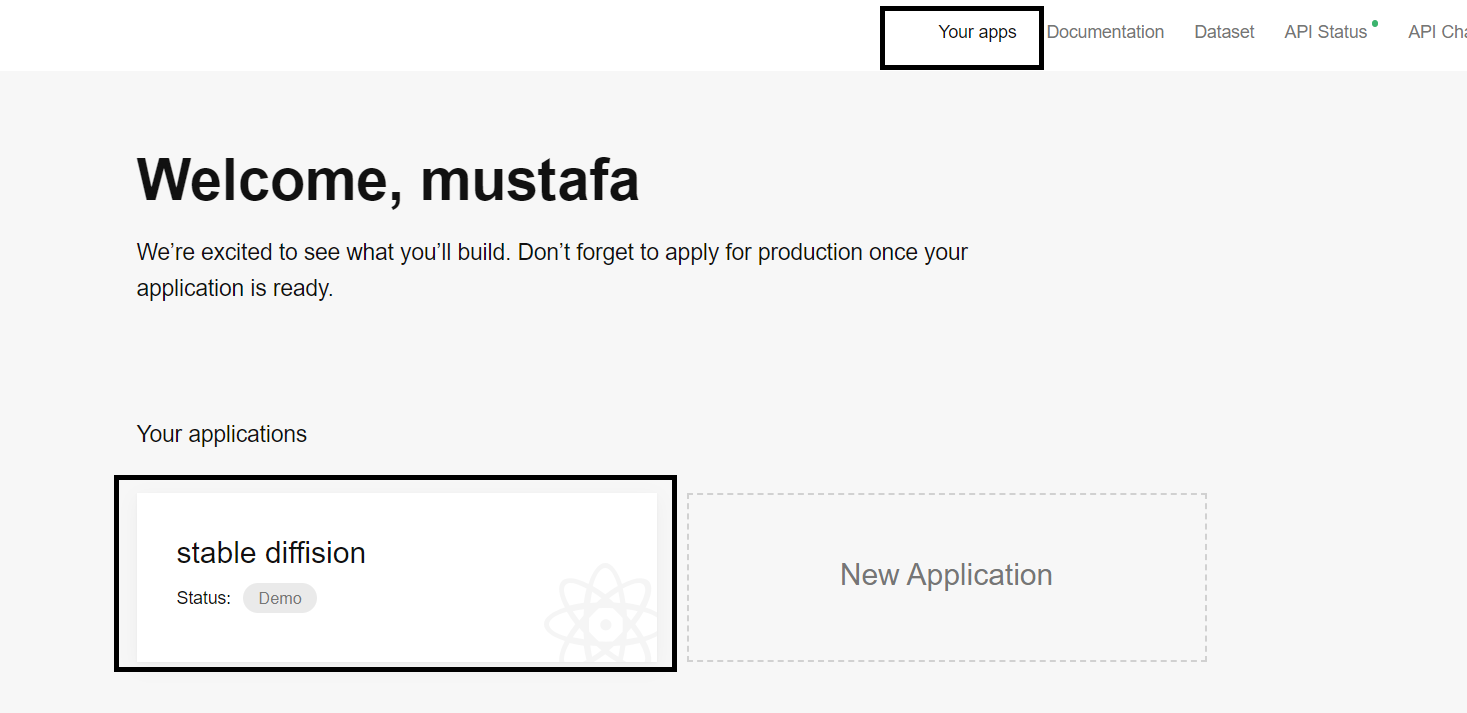
\includegraphics[width=12cm,height=6cm]{app.png}
		\caption{Unsplash app sayfası}
		\label{görsel1}
	\end{figure}
	\begin{figure}[h]
		\centering
		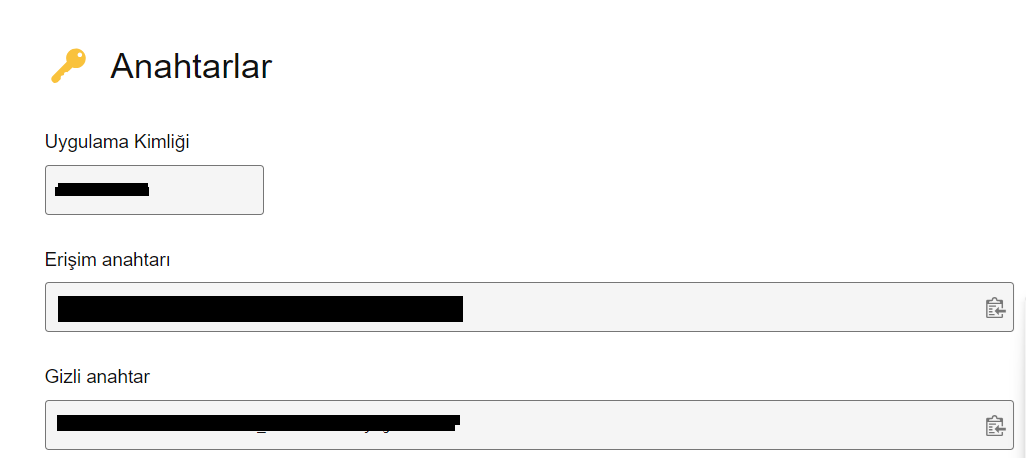
\includegraphics[width=12cm,height=6cm]{unsplashKey.png}
		\caption{proje oluşturma}
		\label{proje}
	\end{figure}
	
	Yukarıdaki \ref{proje} numaralı şekilde görülen anahtarlar kodda gerekli kısımlara eklenerek projede kullanılabilir hale geliyor.
	\newpage
	
	\section{BULGU ve TARTIŞMA(hatalar burada)}
	\textbf{Model eğitim değerleri}
	\begin{figure}[h]
		\centering
		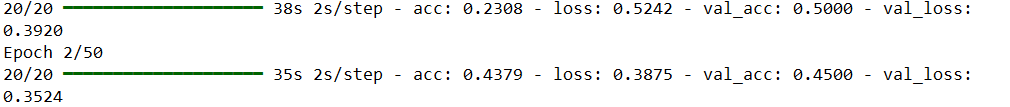
\includegraphics[width=12cm,height=2cm]{epoch1.png}
		\caption{epoch değeri=50 epochun 1. ve 2. değerleri}
		\label{epoch1}
	\end{figure}
	
	\begin{figure}[h]
		\centering
		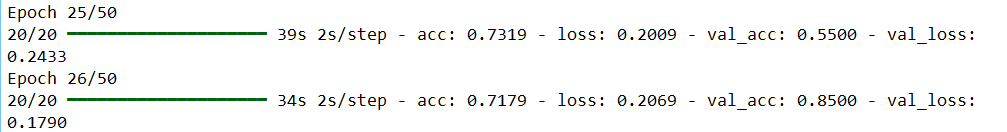
\includegraphics[width=12cm,height=2cm]{epoch2.png}
		\caption{epoch değeri=50 epochun 25. ve 26. değerleri}
		\label{epoch2}
	\end{figure}
	
	\begin{figure}[h]
		\centering
		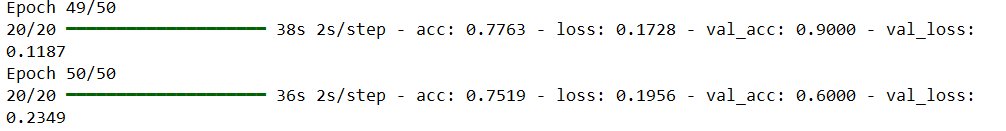
\includegraphics[width=12cm,height=2cm]{epoch3.png}
		\caption{epoch değeri=50 epochun 49. ve 50. değerleri}
		\label{epoch3}
	\end{figure}
	\newpage
	\textbf{Epoch:} Bir epoch, modelin tüm eğitim setini bir kez gördüğü bir eğitim döngüsünü temsil eder. Görselde 50 epoch olduğunu görebilirsiniz, bu da modelin eğitim setini 50 kez gördüğü anlamına gelir.\\
	\textbf{Loss} Loss, modelin tahminleri ile gerçek değerler arasındaki farkın bir ölçüsüdür. Düşük bir loss değeri, modelin daha iyi tahminler yaptığı anlamına gelir. Görselde loss değeri epoch boyunca azalmaktadır, bu da modelin eğitim ilerledikçe daha iyi hale geldiğini gösterir.\\
	\textbf{Accuracy:} Accuracy, modelin doğru tahminlerde bulunma oranını temsil eder. Yüksek bir accuracy değeri, modelin daha iyi performans gösterdiği anlamına gelir. Görselde accuracy değeri epoch boyunca artmaktadır, bu da modelin eğitim ilerledikçe daha fazla doğru tahmin yaptığı gösterir.\\
	\textbf{Val loss:} Val loss, doğrulama seti olarak adlandırılan ayrı bir veri kümesi üzerinde hesaplanan loss değeridir. Doğrulama seti, modelin eğitim setine aşırı uyum sağlamadığından emin olmak için kullanılır. Düşük bir val loss değeri, modelin genelleme yeteneğine sahip olduğunu gösterir, yani eğitim setinde görmediği veriler üzerinde de iyi performans gösterebileceği anlamına gelir. Görselde val loss değeri epoch boyunca azalmaktadır, bu da modelin genelleme yeteneğini geliştirdiğini gösterir.\\
	\textbf{Val accuracy:} Val accuracy, doğrulama seti üzerinde hesaplanan accuracy değeridir. Yüksek bir val accuracy değeri, modelin genelleme yeteneğine sahip olduğunu gösterir. Görselde valaccuracy değeri epoch boyunca artmaktadır, bu da modelin genelleme yeteneğini geliştirdiğini gösterir.
	
	\subsubsection{Word2Vec modeli}
	Word2Vec'in iki ana modeli vardır:\\
	\textbf{CBOW} (Continuous Bag-of-Words): Bu model, bir kelimenin etrafındaki kelimeleri tahmin etmek için kelimenin kendisini kullanır.Daha az veriyle daha hızlı bir şekilde eğitilmesi gereken modeller için daha uygundur.\\
	\textbf{Skip-gram:}Bu model, bir kelimeyi tahmin etmek için etrafındaki kelimeleri kullanır.
	Word2Vec, kelime benzerliği bulma, ilgili kelimeler önerme ve metin sınıflandırma gibi çeşitli NLP görevlerinde kullanılabilir.Daha az gürültülü veriyle daha iyi sonuçlar veren modeller için daha uygundur.\\
	\subsubsection{GloVe(Global Vectors for Word Representation):}
	GloVe, kelimeleri hem yerel hem de küresel istatistikleri kullanarak vektörlere dönüştürür. Yerel istatistikler, kelimelerin kelime bağlam penceresinde birlikteliklerini temsil ederken, küresel istatistikler kelimelerin tüm metin kümesindeki birlikteliklerini temsil eder.
	GloVe, Word2Vec'e kıyasla daha az gürültülü ve daha anlamlı vektörler üretme eğilimindedir. GloVe, kelime benzerliği bulma, duygu analizi ve makine çevirisi gibi çeşitli NLP görevlerinde kullanılabilir.
	
	
	\subsection{Veri kümesi ve kullanılan veriler }
	{\textbf{Veri kümesinin içeriği:}Doğa görselleri}\\
	{\textbf{Veri kümesinin adı:}Landscape - Pictures - litter on forest floor-dataset}\\
	{\textbf{Veri kaynağı:\cite{Landscape-Pictures},\cite{litter-on-forest-floor},\cite{weather-dataset}}\\
		{\textbf{Veri örnekleri:}\\
			
			\begin{figure}[h]
				\centering
				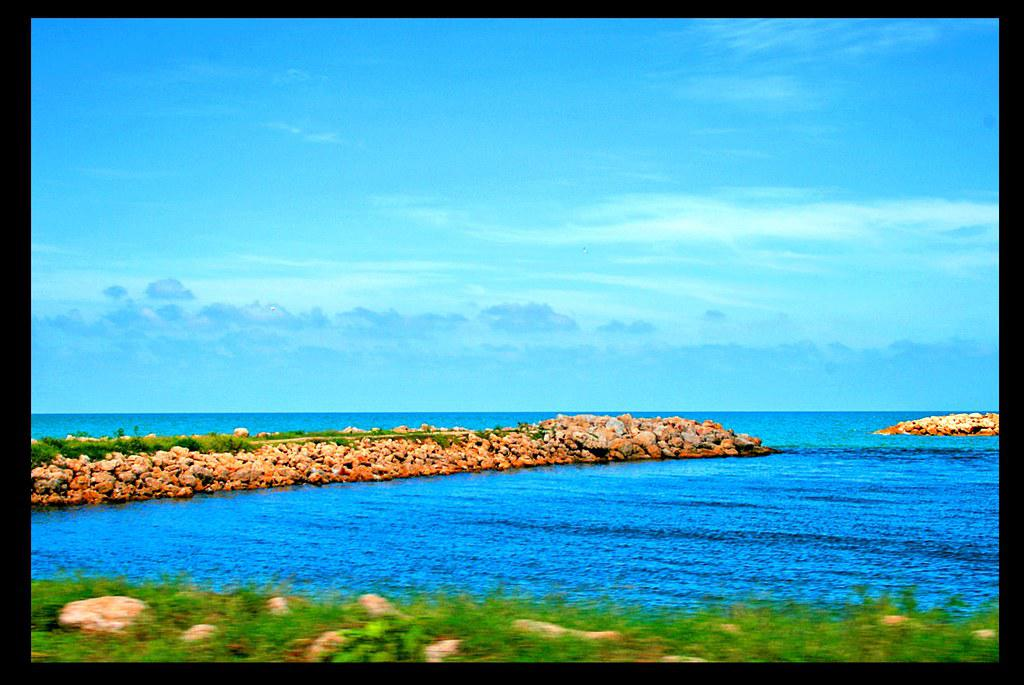
\includegraphics[width=10cm,height=4cm]{00000000_(5).jpg}\\ 	
				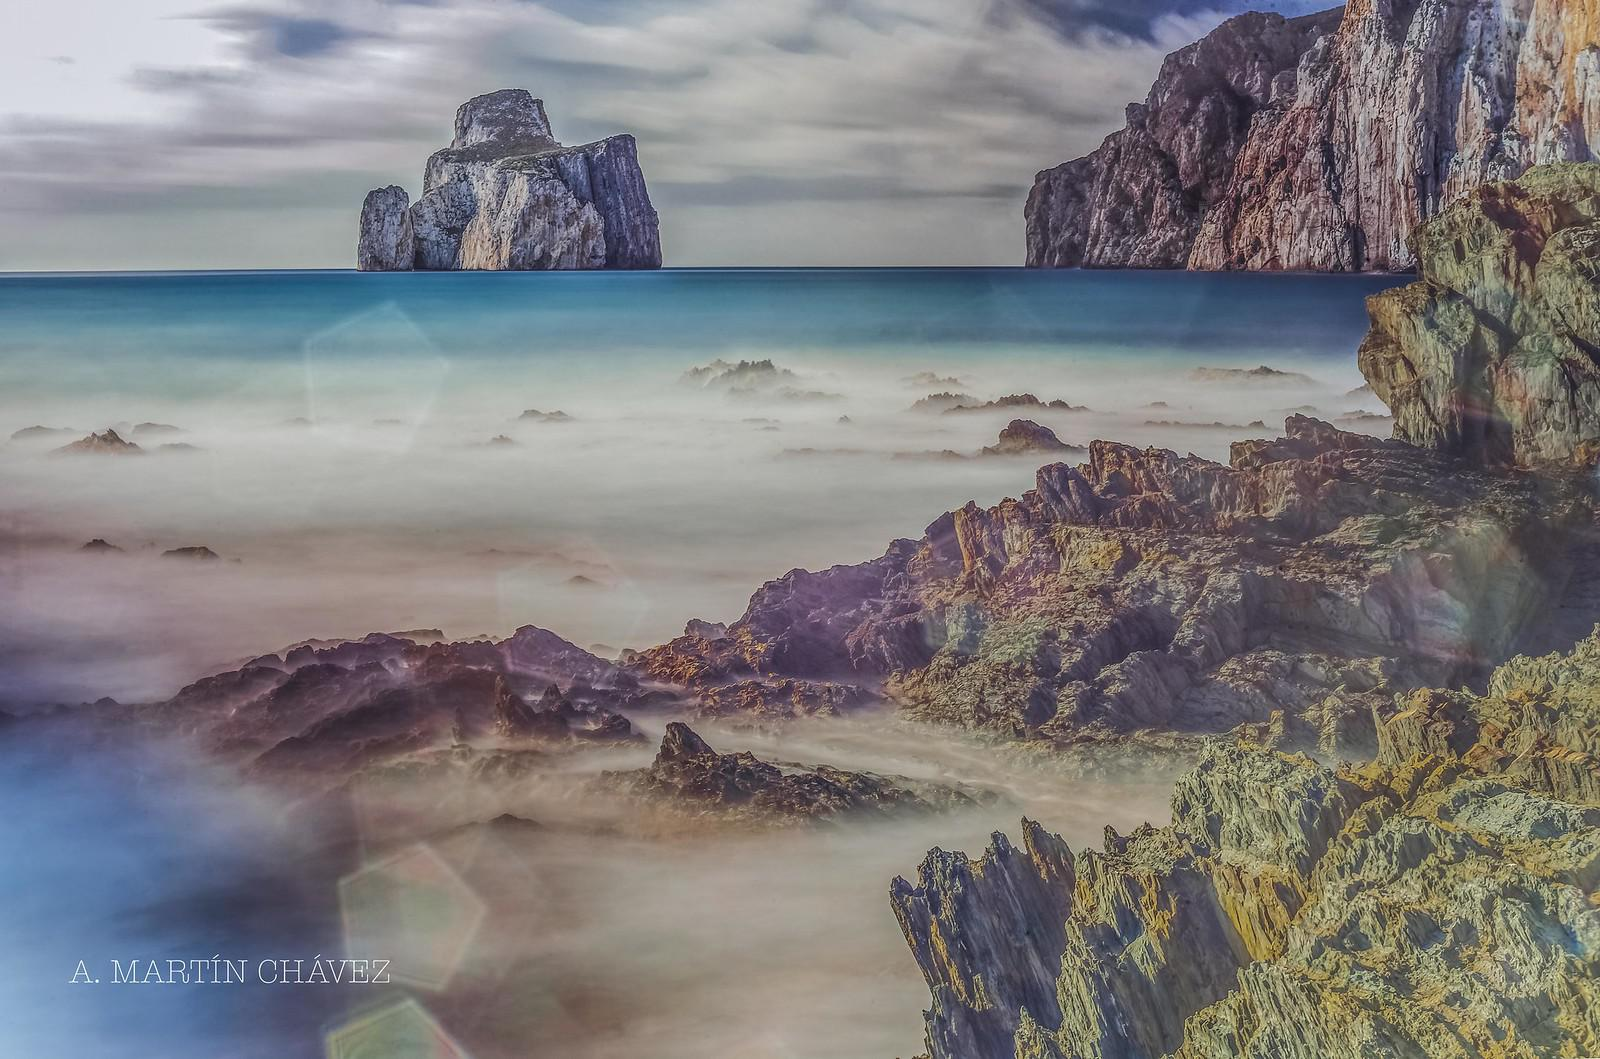
\includegraphics[width=10cm,height=4cm]{00000024_(2).jpg}
				\caption{Landscape-Pictures\cite{Landscape-Pictures}}
				\label{veri}
			\end{figure}
			\subsection{Kaggleden colaba veri çekme}
			Kaggle API'sini kullanarak bilgisayara jayson dosyası içerisinde token indiriyoruz.Burada muhtemel hata alma sebebi olarak bu jason dosyası birden fazla kez indirilirse uyuşmazlık oluyor ve hata alınır.Eğer jason dosyanızda hata alınmamışsa Colab'da veri çekme işlemi için öncelikle Şekil \ref{kaggleToken}'deki Kaggle API anahtarını alıp ve Colab'da koddaki gerekli ayarlamaları yapmak gerekiyor.
			
			\begin{figure}
				\centering
				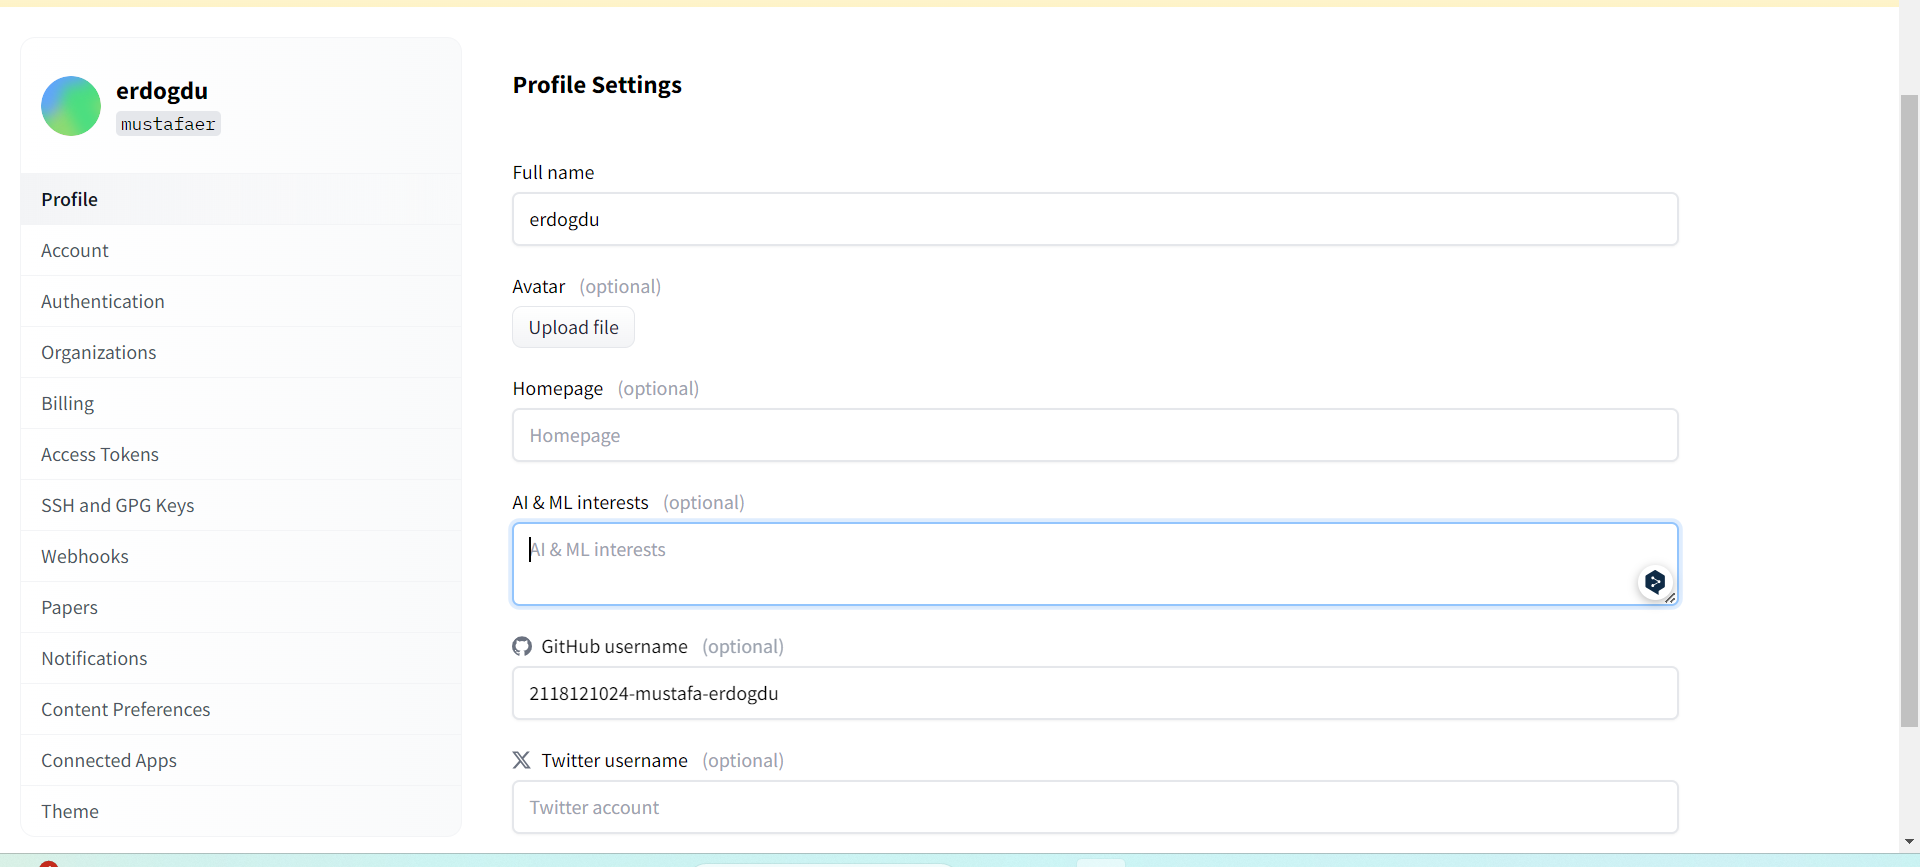
\includegraphics[width=10cm,height=5cm]{huggingFaceToken.png}
				\caption{kaggleToken}
				\label{kaggleToken}
			\end{figure}
			
			\subsection{Colab hugging face bağlama}
			Şekil \ref{huggingFaceToken}'deki hugging face token anahtarını alıp ve Colab'da koddaki gerekli ayarlamaları yapmak gerekiyor.
			\begin{figure}
				\centering
				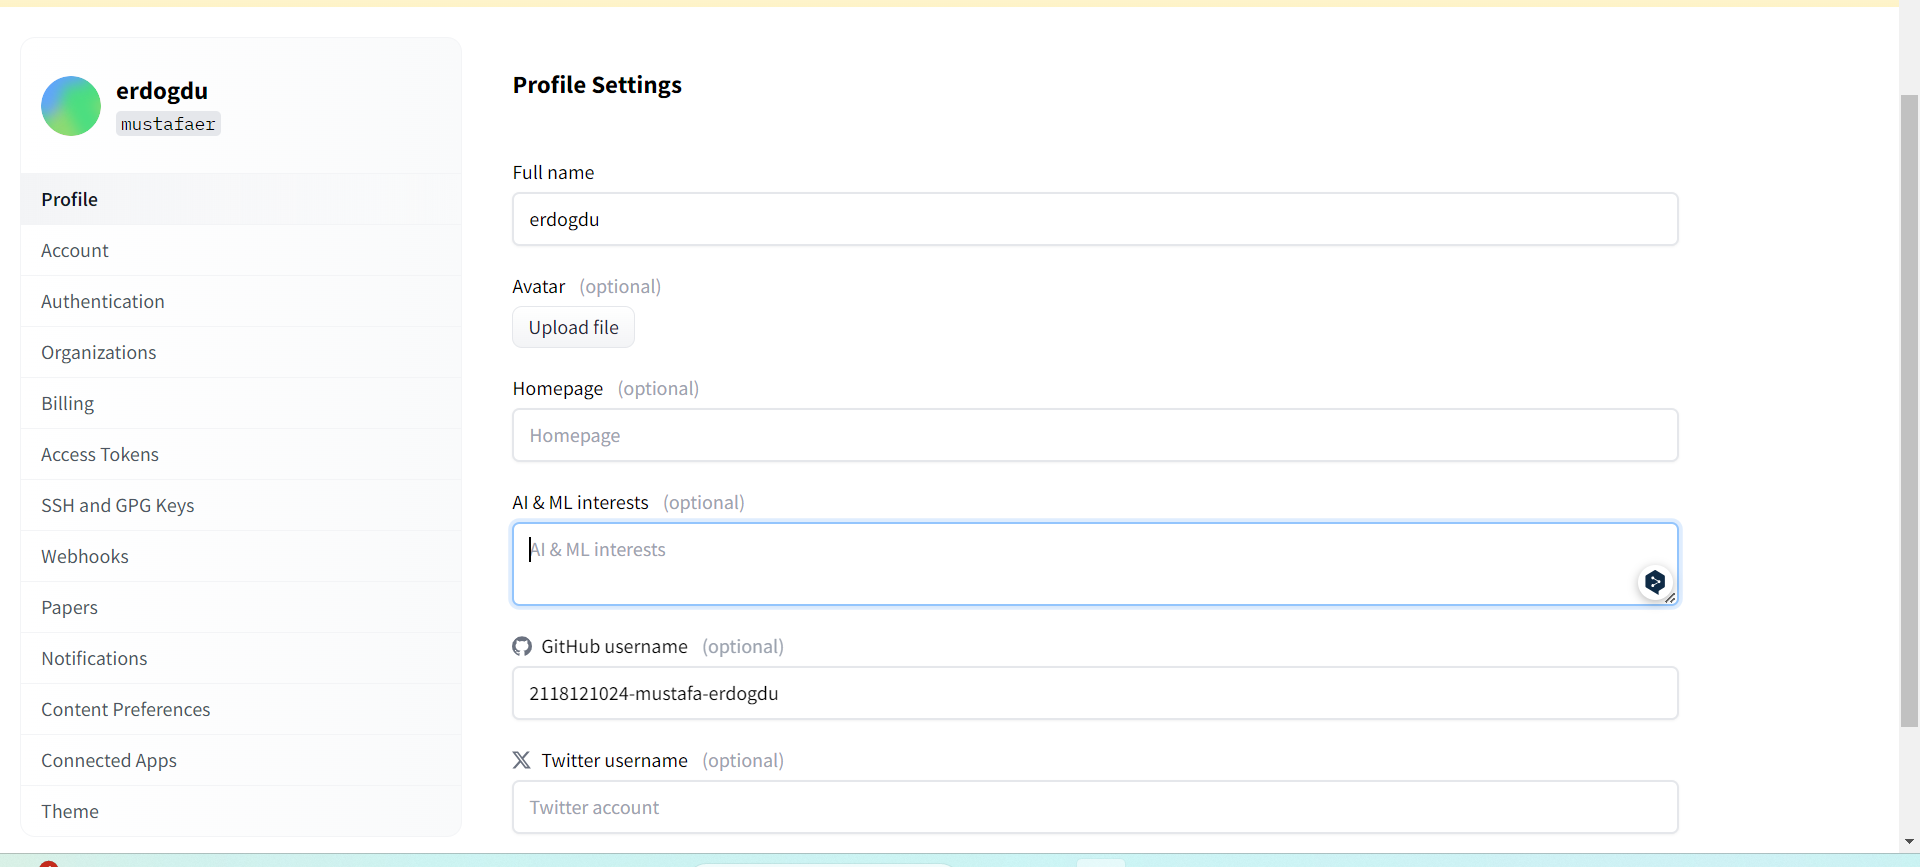
\includegraphics[width=10cm,height=5cm]{huggingFaceToken.png}
				\caption{huggingFaceToken.png}
				\label{huggingFaceToken}
			\end{figure}
			\newpage
			
			Colaba veri çekerken alınabilecek bazı hatalar ve çözümleri,Şekil \ref{webHata}'daki hata giriş yapılmak istenilen web sitesi adresinde giriş yetkilendirmesinin olmadığını belirten bir hatadır.hugging face ile colab e mailleri farklı olursa bu hata alınır. önüne geçmek için mailleri kontrol etmek gerkiyor.
			\\
			
			\begin{figure}
				\centering
				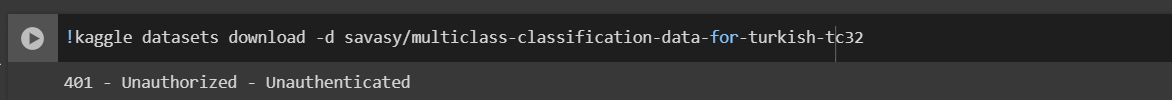
\includegraphics[width=16cm,height=1cm]{webHata.png}
				\caption{webHata\cite{github}}
				\label{webHata}
			\end{figure}
			
			\subsection{Projede karşılaşılabilecek hatalar ve çözümleri}
			\begin{figure}[h]
				\centering
				\includegraphics[width=9cm,height=1cm]{tutarsız_veri.png}
				\caption{hata1}
				\label{hata1}
			\end{figure}
			Şekil \ref{hata1} deki hatanın sebebi veri setindeki metinlerin hepsinin etiketli olmadığından veya etiket değerleri etiketlenmesi gereken veriden fazla olduğu zaman buhata alınır.
			\begin{figure}[h]
				\centering
				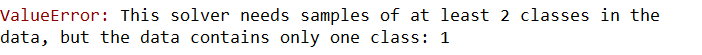
\includegraphics[width=9cm,height=1cm]{verisetiDegerleri.png}
				\caption{hata2}
				\label{hata2}
			\end{figure}	
			Hata \ref{hata2} de görecğimiz üzere word2vec modeli sınıflandırma modeli olduğu için en az iki sınıf olması gerekiyor.
			
			\begin{figure}[h]
				\centering
				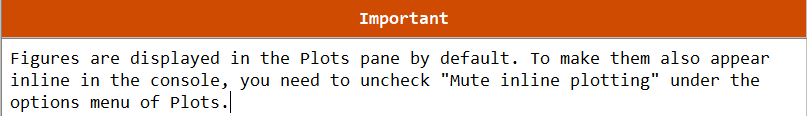
\includegraphics[width=12cm,height=2cm]{görsel oluşturma hatası .png}
				\caption{Görsel oluşturma uyarısı}
				\label{görsel1}
			\end{figure}
			
			\begin{figure}[h]
				\centering
				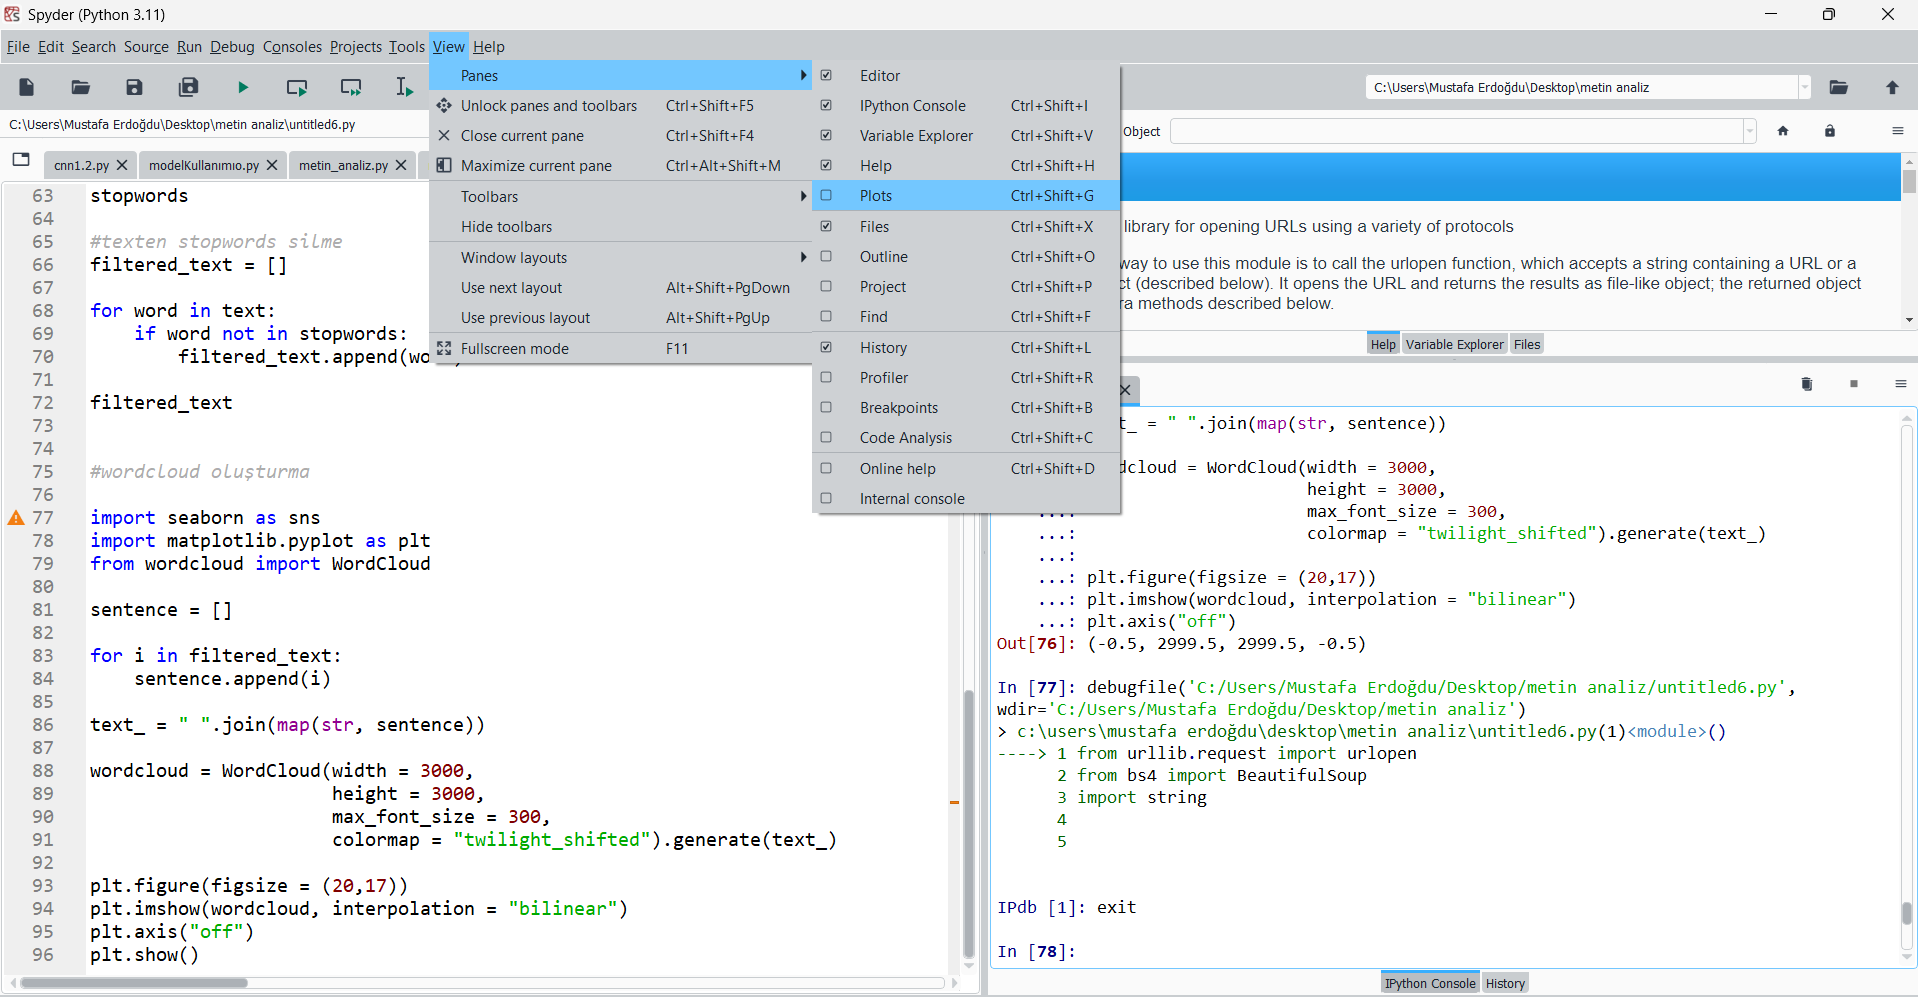
\includegraphics[width=12cm,height=8cm]{grafik görüntüleme.png}
				\caption{Grafik görüntüleme ayarı açılması}
				\label{grafik görüntüleme}
			\end{figure}
			
			\newpage
			Şekil \ref{görsel1}'de alınan uyarı \ref{grafik görüntüleme} numaralı şekilde belirtildiği şekilde grafik görüntüleme ayarları açılır.
			
			
			\begin{figure}[h]
				\centering
				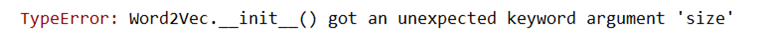
\includegraphics[width=12cm,height=1.5cm]{sürümHatası.png}
				\caption{Size sürüm hatası.}
				\label{size}
			\end{figure}
			şekil \ref{size} 'de alınan hata size ifadesi w2w modelin eski sürümlerinde kullanılıyor.Yeni 
			sürümde vektor size ifadesi kullanılması gerekiyor.
			\begin{figure}[h]
				\centering
				\includegraphics[width=15cm,height=3cm]{apiunsplashhatası.png}
				\caption{api unsplash hatası}
				\label{hata1}
			\end{figure}
			Yukarıdaki \ref{hata1} numaralı şekilde görülen hata erişim anahtarının hatalı girilmesinden kaynaklanıyor.Hatanın düzeltilmesi için "Unsplash API kullanımı ve proje oluşturma" adımını inceleyebilirsiniz.
			
			
			\section{SONUÇ}
			10 haftalık bir süreyi kapsayan bu projede, Stable Video Diffusion modelinin temel prensipleri ve kullandığı teknolojiler (örneğin, derin öğrenme, difüzyon modelleri) araştırılarak benzer teknolojiler ve çalışmalar (örneğin, DALL-E 2,gail) ile karşılaştırıldı. Bu sayede, Stable Video Diffusion modelinin güçlü ve zayıf yönleri belirlenerek, bu modele benzer bir modelin geliştirilmesine zemin hazırlandı.Stable diffision modelini farklı bir versiyonu gelişltirilmeye çalışıldı. Proje kapsamında, modelin metin açıklamalarını doğru şekilde yorumlayabilmesi için gerekli veri setleri ve eğitim yöntemleri belirlendi, farklı manzara türlerini ve farklı metin formatlarını desteklemesi için gerekli geliştirmeler yapıldı. 
			
			
			\cite{wang2018assessment}
			
			\subsection{Gelecekte yapılması planlanan çalışmalar nelerdir?} 
			Gelecek süreçte hedeflenen başarım, kullanıcının girdiği metinden metin vektörü elde edilip doğrudan bir manzara resmi oluşturabilen bir model inşa edilmiş olacak ve bu modelin farklı metin açıklamalarına ve parametrelere karşı test edilerek, modelin oluşturduğu resimlerin kalitesinin ve çeşitliliğinin değerlendirilmesi ve modelin sınırlamalarının belirlenmesi gibi işlemler tamamlanacaktır. Metinden görsel üretme işlemi stable diffision aksine doğruden kelime vektörleri ile sağlanacak.
			%Kaynakçayı
			\bibliographystyle{ieeetr}
			\bibliography{references.bib} 
			
			
			
			
			
			
			
			
			
			
		\end{document}
